% %%%%%%%%%%%%%%%%%%%%%%%%%%%%%%%%%%%%%%%%%%%%%%%%%%%%%%%%%%%%%%%%% SECTION FIVE
% %%%%%%%%%%%%%%%%%%%%%%%%%%%%%%%%%%%%%%%%%%%%%%%%%%%%%%%%%%%%%%%%%%%%%%%%%%%%%%
\section{Mid-Side}

Harvey Fletcher, fisico americano, nel 1934 firma uno degli articoli che
compongono un testo cardine per la storia della tecnologia sonora
“\emph{Symposium on Auditory Perspective}”, sulla percezione e la trasmissione
della musica dal vivo, che inizia con le seguenti parole:

\begin{quote}
In this electrical era one is not surprised to hear that orchestral music can be
picked up in one city, transmitted a long distance, and reproduced in another.
Indeed, most people think such things are commonplace. They are heard every
night on the radio. However, anyone who appreciates good music would not admit
that listening even to the best radio gives the emotional thrill experienced in
the concert hall. \cite{hf34}
\end{quote}

Oggi abbiamo perso ogni scintilla di “quell'era elettrica”, anche quella che ha
suscitato la fiamma di interesse nell'ascolto della musica orchestrale
attraverso la trasmissione.

%, o quella che ha suscitato la fiamma di interesse
% nell'ascolto della musica orchestrale, o quella dell'interesse nell'ascolto o,
% molto più semplicemente, la fiamma dell'di interesse. Cento anni dopo quella
% “era” siamo scimmie. Dobbiamo considerare questo fallimento. Inadempienza. Dobbiamo considerare che
% un libro, anche il più inadeguato, in quanto oggetto di pensiero ha potere, come
% dimostrato nell'introduzione, che potrebbe essere il potere di distruggere.

Nel 1964, Paul W. Klipsch introdusse la ristampa del “\emph{Symposium}”:

\begin{quote}
The following paper is a reprint of one of the most important papers in the
field of audio. Fundamentals do not change. The laws of physics endure. In
reprinting the Symposium, the fundamentals are restated. \cite{sap1964}
\end{quote}

Il testo di Fletcher \cite{hf34} è datato 1934, un anno dopo l'approvazione
del brevetto Blumlein che descrive il concetto fondamentale di trasmissione e
registrazione del suono \emph{Mid-Side}. In quell'epoca gli interessi commerciali e
quelli di ascolto erano intrecciati, in una forma \emph{stereo} solida.

Parlando di orecchie e attività cerebrali per determinare la direzione di una
fonte Blumlein ha scritto:

\begin{quote}
…it is fairly well established that the main factor having effect are phase
differences and intensity differences between the sounds reaching the two ears,
the influence with each of these has depending upon the frequency of the sounds
emitted. For low frequency sound waves there is little or non difference in
intensity at the two ears but there is a marked phase difference. For a give
obliquity of sound the phase difference is approximately proportional to
frequency, representing a fixed time delay between sound arriving at the two
ears, by noting which there is a phase difference of $\pi$ radians or more
between sound arriving at the two ears from a source located on the line joining
them: but above such frequency if phase difference were the sole feature relied
upon for directional location there would be ambiguity in the apparent position
of the source. At the stage however the head begins to became effective as a
baffle and causes noticeable intensity difference between the sounds reaching
the two ears, and it is by noting such intensity difference that brain
determines direction of sounds at higher frequencies\footnote{\cite{ab58} - ...è abbastanza
accertato che il fattore principale sia dovuto alle differenze di fase e di
intensità tra i suoni che raggiungono le due orecchie, l'influenza con ognuna di
queste differenze ha a seconda della frequenza dei suoni emessi. Per le onde
sonore a bassa frequenza c'è poca o nessuna differenza di intensità alle due
orecchie ma c'è una marcata differenza di fase. Per dare un'obliquità del suono,
la differenza di fase è approssimativamente proporzionale alla frequenza, che
rappresenta un ritardo fisso tra il suono che arriva alle due orecchie, notando
che c'è una differenza di fase di $\pi$ radianti o più tra il suono che arriva
alle due orecchie da una sorgente situata sulla linea che le unisce: ma al di
sopra di tale frequenza se la differenza di fase fosse l'unica caratteristica
su cui si basava per la posizione direzionale, ci sarebbe ambiguità nella
posizione apparente della sorgente. Tuttavia, nella fase in cui la testa inizia
a diventare efficace come un deflettore e causa una notevole differenza di
intensità tra i suoni che raggiungono le due orecchie, ed è notando tale
differenza di intensità che il cervello determina la direzione dei suoni a
frequenze più alte.}.
\end{quote}

Sulla base della conoscenza dei meccanismi sopra esposti Blumlein ha formulato
la maggior parte dei principi fondamentali impressi nella storia della stereofonia.
L'approccio più semplice descritto permette di ottenere semplici differenze di
livello nella riproduzione dagli altoparlanti, percepite come differenze di
livello e di fase dalle orecchie. Per ottenere questo tipo di segnale sono
necessari almeno due microfoni posizionati tra loro vicinissimi, allineati
verticalmente, in modo da non avere alcun ritardo (orizzontale) tra i canali.
Questa configurazione definita \emph{coincidente} è l'ideale per alimentare
gli altoparlanti con differenze pure di ampiezza tra i canali. Una delle tipiche
tecniche di ripresa stereofonica per coppia coincidente prende proprio il nome
da Blumlein: due microfoni bidirezionali, figura-8 quindi a gradiente di pressione,
angolati tra loro di $\pm45$ gradi, in modo da avere un angolo retto tra loro.

Tuttavia, come esposto nel brevetto, i soli microfoni disponibili a Blumlein nei
suoi primi esperimenti erano dinamici non-direzionali a pressione. Coppie
stereofoniche coincidenti con microfoni di questo tipo non sono possibili, in
quanto il loro allineamento verticale produrrebbe due segnali identici, che non
descriverebbero stereofonia. È necessaria quindi una distanza tra i due microfoni.
Due microfoni non-direzionali distanziati anche poco tra loro sono in grado di
produrre segnali quasi identici in ampiezza ma diversi in fase. Blumlein quindi
si concentra su una strategia per produrre anche una differenza di ampiezza tra
i due microfoni, inserendo un blocco di legno tra i due microfoni e progettando
una matrice elettrica che mettesse in relazione i due segnali in modo da
produrre le giuste differenze di ampiezza nell'altoparlante. Il prodotto di tale
ricerca fu la matrice di somma e differenza alla base della tecnologia
\emph{Mid-Side}.

\begin{quote}
\ldots a system of sound transmission wherein the sound
is receive by two or more microphones, wherein at low frequencies difference in
the phase of sound pressure at the microphone is reproduced as difference in
volume at the loud speaker. [\ldots] two microphones transmitted over individual
channels are adapted to interact [\ldots] consisting in half of the sum and half
of the difference respectively of the original \cite{ab58}
\end{quote}

\begin{figure*}[b!]
    \centering
    \begin{subfigure}[t]{0.48\textwidth}
        \centering
        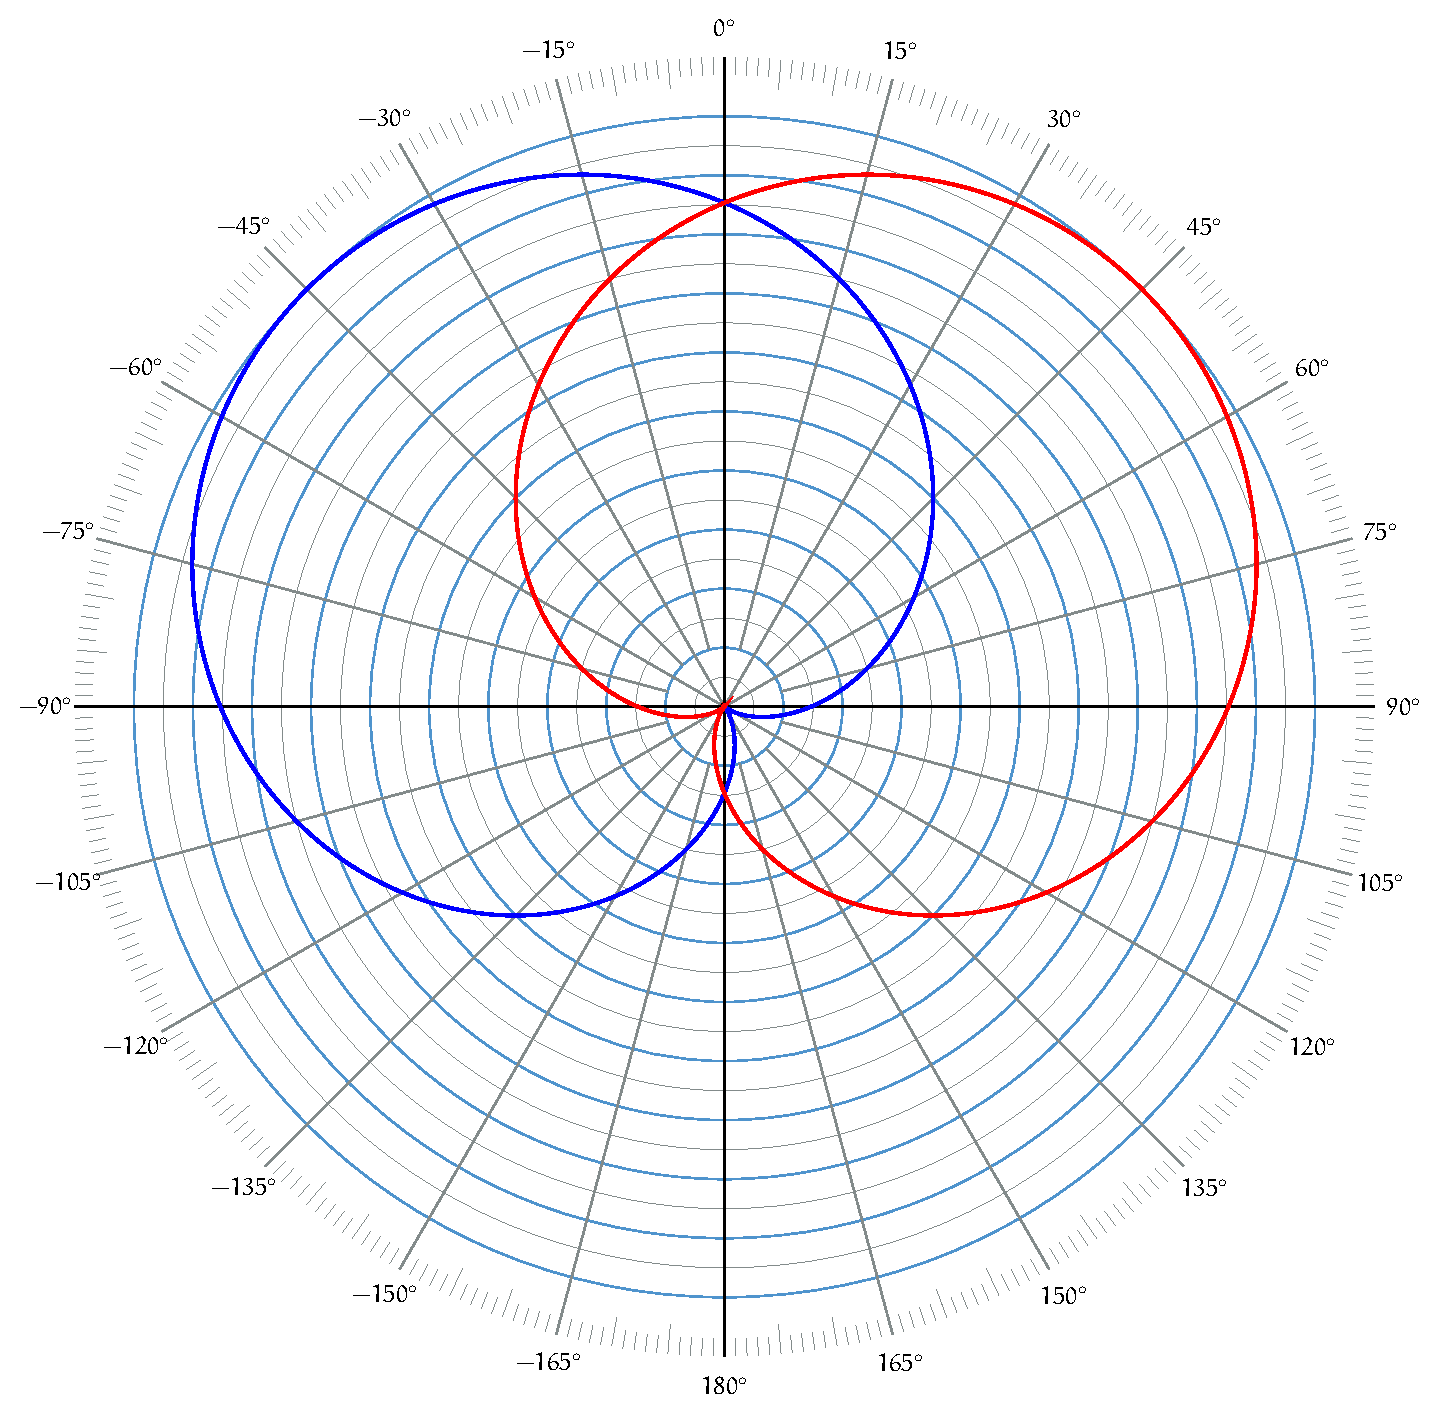
\includegraphics[height=6cm]{microphone-polar-patterns/xy90}
        \caption[]{Coppia stereofonica coincidente di cardioidi angolati di 90 gradi tra loro in entrata alla matrice.}% \\ Eq: $1(x)$}
        \label{pol:xy90ms}
    \end{subfigure}%
    ~
    \begin{subfigure}[t]{0.48\textwidth}
        \centering
        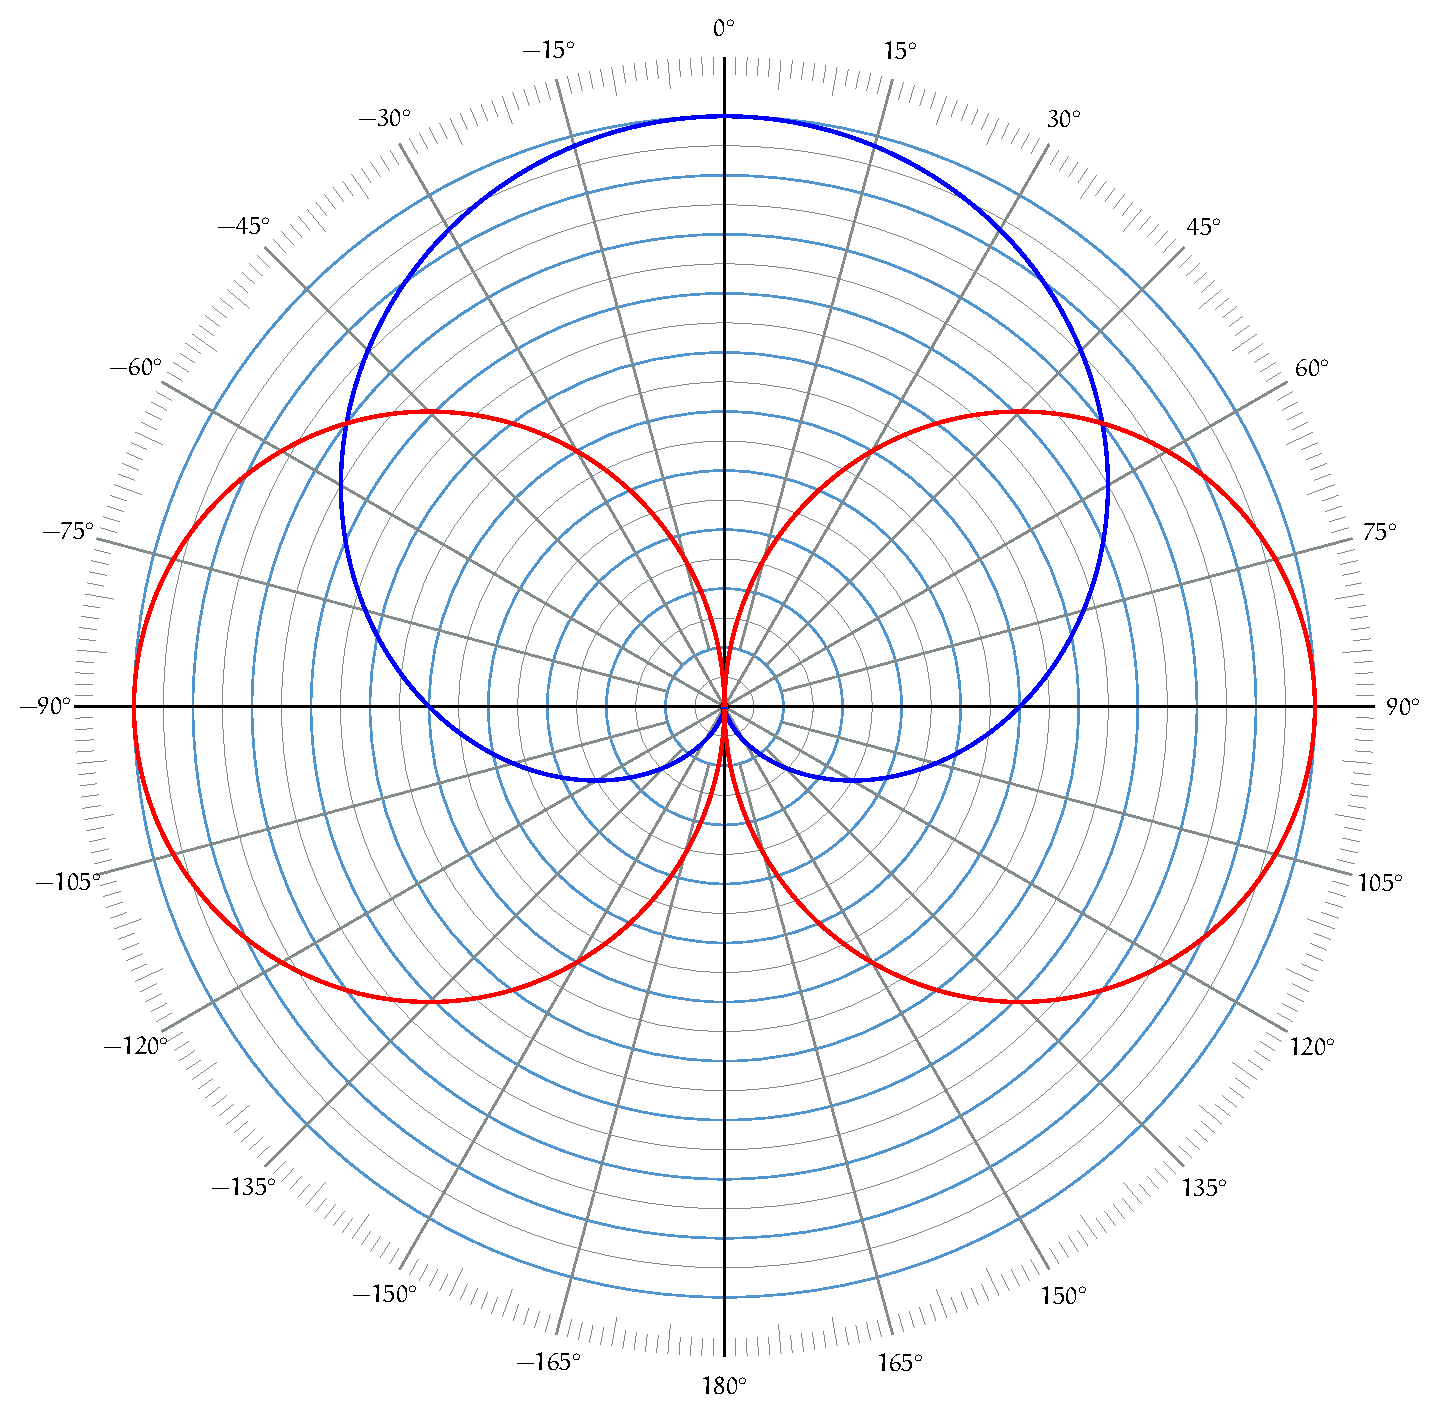
\includegraphics[height=6cm]{microphone-polar-patterns/midside}
        \caption[]{Le componenti \emph{Mid-Side} in uscita.}% \\ Eq: $0.75(x)+0.25(x\cos\theta)$}
        \label{pol:midsidems}
    \end{subfigure}
    \caption[]{Rappresentazione polare ideale del transito di una coppia \emph{xy90}
    attraverso la matrice e relativa rappresentazione d'uscita \emph{Mid-Side}.}
    \label{pol:msmatrix}
\end{figure*}

La matrice di Blumlein di somma e differenza tra i segnali è bidirezionale.
Quando il canale sinistro e destro di una coppia stereofonica passa attraverso
la matrice, la somma di entrambi i canali fornisce il segnale \emph{Mid}
contenente solo le componenti in fase, mentre la differenza produce il segnale
\emph{Side} laterale contenente solo componenti non in fase tra loro. Quando
sono le componenti \emph{Mid-Side} a transitare attraverso la matrice, la somma
di \emph{Mid} e \emph{Side} fornisce la correlazione tra fase sinistra e ampiezza,
mentre la differenza produce la correlazione tra fase negativa a ampiezza.

Di seguito il codice \emph{Faust} per la matrice somma e differenza.

%--------------------------------------------
%----------------larghezza massima del codice
\begin{lstlisting}
nsum = 0.5*(_+_);
ndif = 0.5*(_-_);
sdmx = _,_ <: nsum, ndif;
\end{lstlisting}

\begin{figure}[ht]
  \centering
  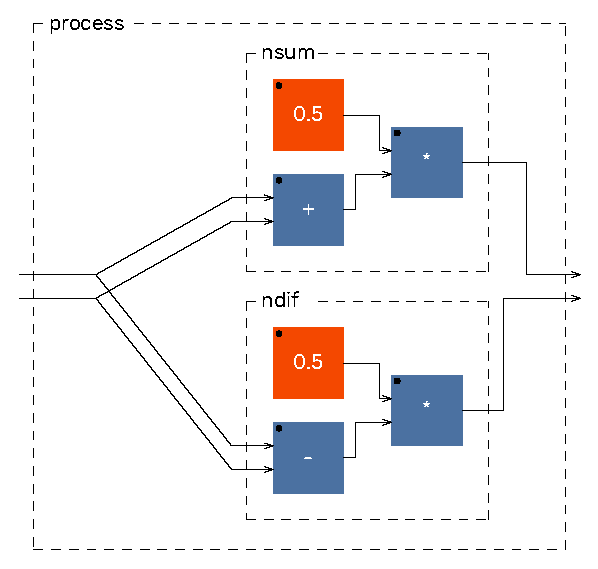
\includegraphics[]{CAPITOLI/0300/IMG/sdmx}
  \caption[]{Matrice somma e sottrazione.}
  \label{bd:sdmx}
\end{figure}

%%%%%%%%%%%%%%%%%%%%%%%%%%%%%%%%%%%%%%%%%%%%%%%%%%%%%%%%%%%%%%%%%%%% SECTION SIX
%%%%%%%%%%%%%%%%%%%%%%%%%%%%%%%%%%%%%%%%%%%%%%%%%%%%%%%%%%%%%%%%%%%%%%%%%%%%%%%%
\subsection{Mid-Side \emph{mic}}
\label{subsec:msmic}

\begin{figure}[b!]
\centering
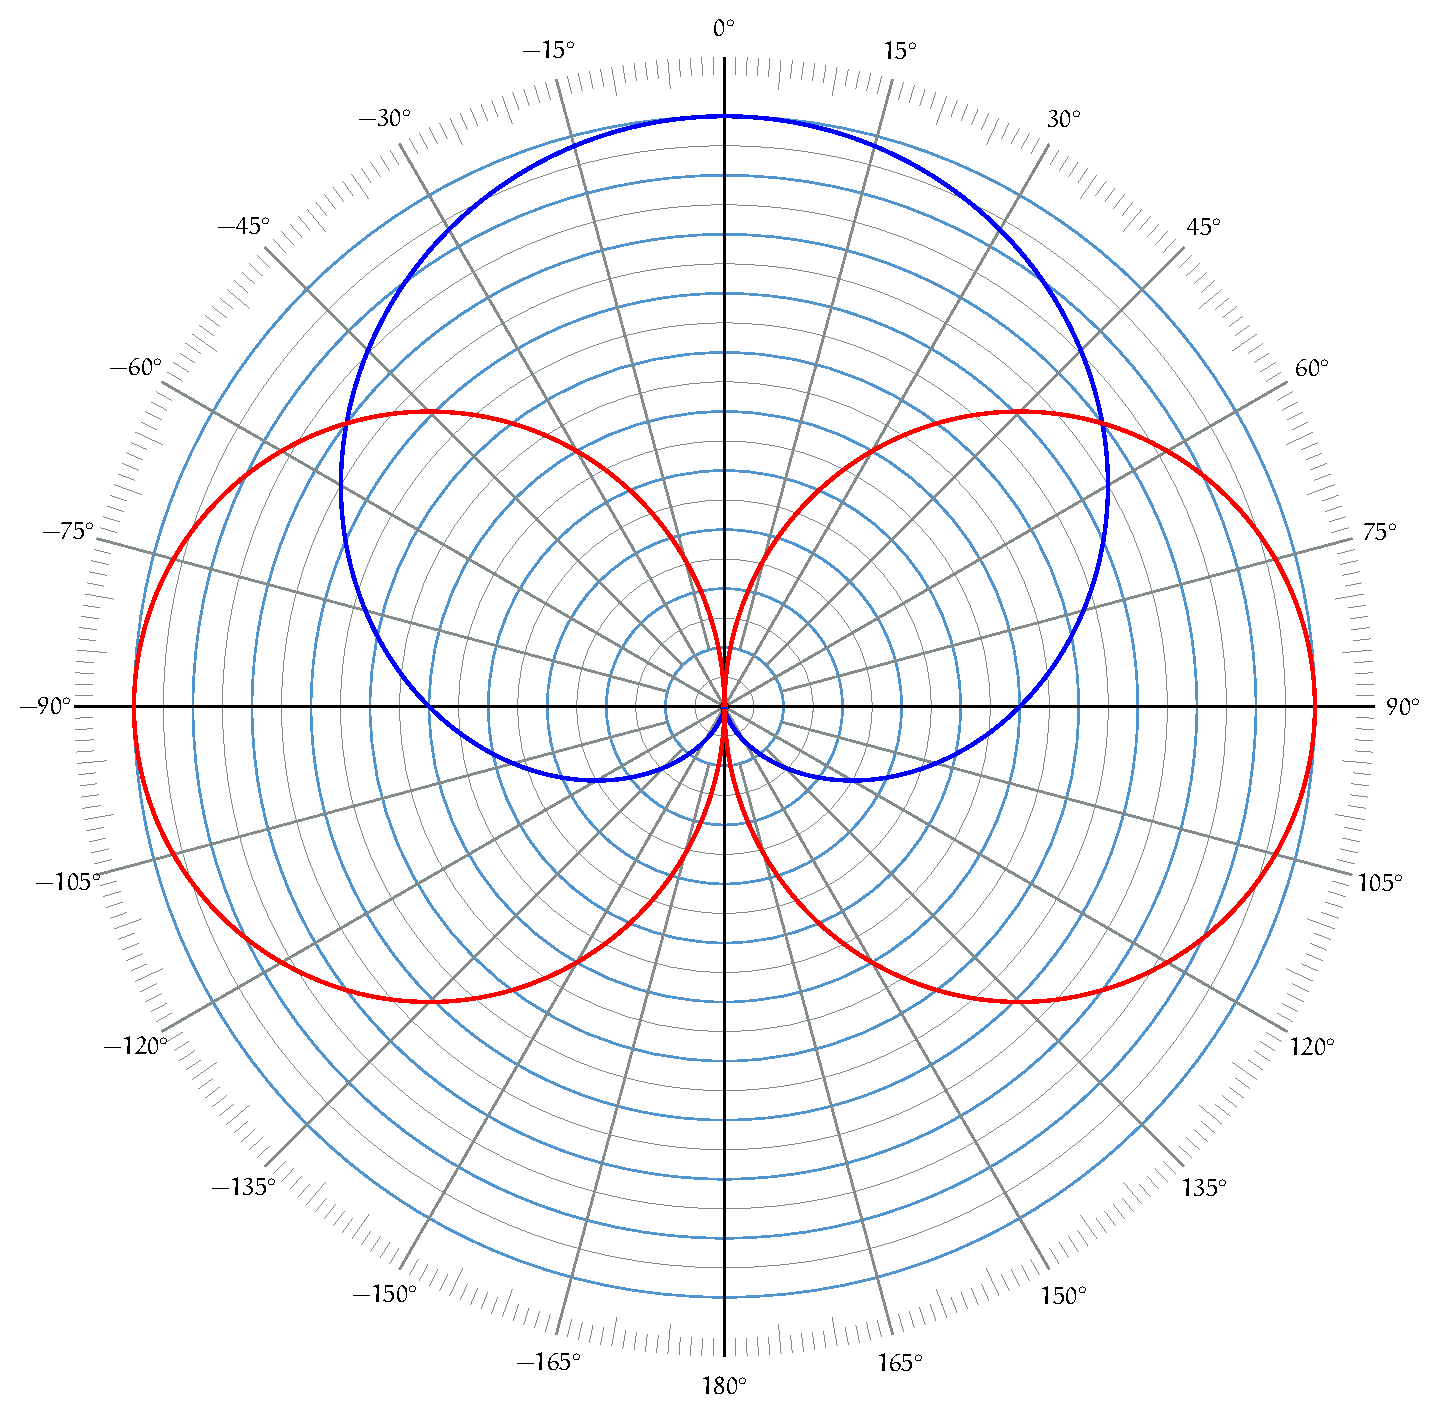
\includegraphics[width=0.99\columnwidth]{microphone-polar-patterns/midside}
\caption[]{Rappresentazione ideale della coppia stereofonica Mid-Side costituita da
da un microfono direzionale cardioide a gradiente di pressione mediante la sua
equazione polare: $cpg = 0.5(x) + 0.5(x\cos\theta)$ (\emph{cardioid pressure
gradient}) e da un microfono bidirezionale a gradiente di
pressione mediante la sua equazione polare: $bpg = x\cos\theta$
(\emph{bidirectional pressure gradient}). Nella tecnica microfonica di registrazione
Mid-Side il microfono cardioide convenzionalmente viene registrato nel primo canale,
mentre il segnale del microfono bidirezinale viene registrato nel secondo canale.}
\label{polar:midsidemic}
\end{figure}

La produzione di un segnale \emph{Mid-Side} come quello in uscita dalla matrice
somma e sottrazione può essere ottenuta dal posizionamento diretto di una coppia
di microfoni aventi caratteristiche polari adeguate. Il segnale \emph{Mid} è
generalmente prodotto da un microfono direzionale cardioide puntato verso il fronte
stereofonico, mentre il segnale \emph{Side} è generato da un microfono
bidirezionale puntato lateralmente, offrendo al fronte il punto di massimo
annullamento. I due microfoni devono essere allineati verticalmente in modo da
risultare orizzontalmente coincidenti.


%%%%%%%%%%%%%%%%%%%%%%%%%%%%%%%%%%%%%%%%%%%%%%%%%%%%%%%%%%%%%%%%%%%% SECTION SIX
%%%%%%%%%%%%%%%%%%%%%%%%%%%%%%%%%%%%%%%%%%%%%%%%%%%%%%%%%%%%%%%%%%%%%%%%%%%%%%%%
\subsection{Mid-Side \emph{panner}}
\label{subsec:mspanner}

La coppia stereofonica di segnali \emph{Mid-Side} è stata descritta finora come
risultante della matrice somma e sottrazione applicata ad un segnale stereofonico
oppure come segnale prodotto da una coppia di microfoni aventi caratteristiche
oppurtune. Analizziamo ora un terzo sistema in grado di generare una coppia
\emph{Mid-Side} attraverso un sistema di panning.

Il canale frontale \emph{Mid} è comunemente descritto da un microfono cardioide.
Sappiamo che la componente cardioide, come moltre altre figure polari, può
essere risultante da una combinazine misurata di
componenti non-direzionale e bidirezionale.

\begin{equation}
m(x,p,\theta) = (p*x) + ((1-p)*(x\cos\theta)
\label{eq:mid}
\end{equation}

Dove $x$ è il segnale di ingresso, $p$ è il coefficiente di ampiezza che regola
il rapporto di peso tra le due componenti, $0.5$ per ottenere la figura polare
cardioide, $\theta$ è la direzione di impatto angolare espressa in radianti.

La componente \emph{Side} è costituita dalla sola componente bidirezionale.

\begin{equation}
s(x,\theta) = x*(sin(\theta))
\label{eq:side}
\end{equation}

Il codice \emph{Faust} per la costruzione di un \emph{Mid-Side Panner} è
molto simile alle equazioni che descrivono le due figure polari.

%--------------------------------------------
%----------------larghezza massima del codice
\begin{lstlisting}
mspan(x,p,rad) = m,s
with{
  m = (p*x)+((1-p)*(x*cos(rad)));
  s = x*(sin(-rad));
};
\end{lstlisting}

I due segnali in uscita dal panner non possono essere inviati direttamente ad un
sistema di ascolto basato sui due canali sinistra-destra, devono necessariamente
passarli attraverso la matrice somma e differenza ottenere ciò che Blumlein
descrive come la differenza di ampiezza nei segnali degli altoparlanti
ottenuta dalle differenze di fase.

% %--------------------------------------------
% %----------------larghezza massima del codice
% \begin{lstlisting}
% mspan_lr(x,p,rad) = mspan(x,p,rad) : sdmx;
% \end{lstlisting}

\begin{figure}[t]
\centering
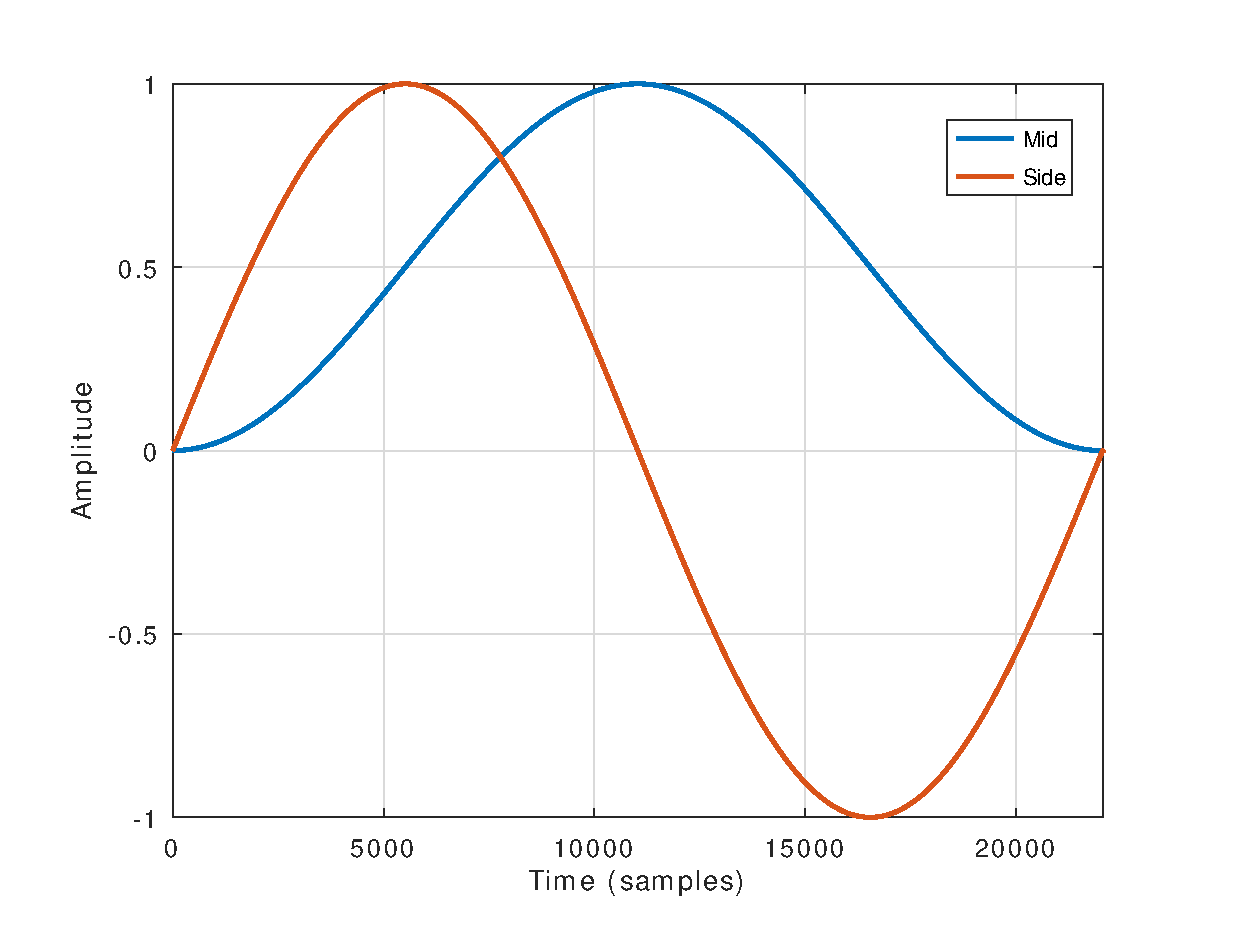
\includegraphics[width=0.99\columnwidth]{CAPITOLI/0300/IMG/mspan}
\caption[]{Mid-Side \emph{panner}. Il grafico mostra la risposta del \emph{panner} ad una
variazione di 360 gradi da sinistra (-180 gradi) a destra (180 gradi). La linea
rossa mostra la bipolarità del segnale correlata alle informazioni angolari. La
linea blu descrive variazioni di ampiezza (sempre con fase positiva) in
relazione alle informazioni angolari. Il grafico mostra l'evidenza della percezione
zero su entrambi gli estremi $\pm180$ gradi, dove cardioide e figura-8 si annullano.}
\label{fig:mspan}
\end{figure}

% La procedura di costruzione dell'algoritmo del \emph{Mid-Side Panner} è completa.
% Il seguente codice di \emph{Faust} descrivo il panner completo di interfaccia
% grafica.

%-----------------------------------------------------------
%-------------------------------larghezza massima del codice
\begin{lstlisting}
//----------------------------------- DEGREES TO RADIANS ---
deg2rad = *(ma.PI/180);
//----------------------------------------------- PANPOT ---
rad = vslider("[02]Azimuth[style:knob]", 0,-180,180,0.1) :
      deg2rad : si.smoo;
//--------------------------------------------- P FACTOR --–
p = vslider("[01]P[style:knob]", 0.5,0,1,0.01) : si.smoo;
//--------------------------------------------- MID-SIDE --–
midside(x,p,rad) = m,s
  with{
    m = (p*x)+((1-p)*(x*cos(rad)));
    s = x*(sin(-rad));
};
//-------------------------------- MS MATRIX DESCRIPTION ---
nsum = 0.5*(_+_);
ndif = 0.5*(_-_);
sdmx = _,_ <: nsum, ndif;
//----------------------------------------- MS2LR MATRIX ---
mspan_lr(x,p,rad) = midside(x,p,rad) : sdmx;
process = os.osc(1000), p, rad : mspan_lr;
\end{lstlisting}
